% Created 2020-04-20 Mon 12:19
% Intended LaTeX compiler: pdflatex
\documentclass[11pt]{article}
\usepackage[utf8]{inputenc}
\usepackage[T1]{fontenc}
\usepackage{graphicx}
\usepackage{grffile}
\usepackage{longtable}
\usepackage{wrapfig}
\usepackage{rotating}
\usepackage[normalem]{ulem}
\usepackage{amsmath}
\usepackage{textcomp}
\usepackage{amssymb}
\usepackage{capt-of}
\usepackage{hyperref}
\author{Aleksandr Petrosyan}
\date{\today}
\title{Project Diary for "Cosmological parameter estimation using Bayesian accelerated Machine learning"}
\hypersetup{
 pdfauthor={Aleksandr Petrosyan},
 pdftitle={Project Diary for "Cosmological parameter estimation using Bayesian accelerated Machine learning"},
 pdfkeywords={},
 pdfsubject={},
 pdfcreator={Emacs 26.3 (Org mode 9.1.9)}, 
 pdflang={English}}
\begin{document}

\maketitle
\tableofcontents

This file contains the notes and the project diary for the
aforementioned project. The diary comes first. If specified, the
timestamp on the notes is when the note was originally written.


\section{Michaelmas}
\label{sec:orgb16a5e7}
\subsection{Week 3}
\label{sec:org88e5f7e}
\subsubsection{{\bfseries\sffamily DONE} Meet Dr Handley}
\label{sec:org70dbecc}
Discussed the project. Talked about Nested
Sampling. Applications to Machine Learning.

Primordial power spectrum, and discretisation. This causes the
Fourier transform \emph{multipole plot} of the CMB. Multipole
moment related to size of blotches on the picture.

\subsection{Week 4}
\label{sec:org8ce2216}
\subsubsection{{\bfseries\sffamily DONE} Read the Abstract. ,}
\label{sec:org2666e03}
Read \href{https://arxiv.org/abs/0803.4089}{Bayes in the sky} Read about Bayesian analysis. 
\(\Omega_{k}\) more significant than thought. 
\subsubsection{{\bfseries\sffamily DONE} Install PolyChord, Cobaya, anesthetic, CosmoChord.}
\label{sec:orgf05707d}
Issues with Mac OS X/XCode. 
GFortran was installed but not on PATH. 
PolyChord not Pip installable. 
\begin{verbatim}
C=cc CXX=cxx python setup.py install —user
\end{verbatim}
doesn't work on OS X. 

Use Python3. 
\subsubsection{{\bfseries\sffamily DONE} EMail will and create a PR to fix Python version.}
\label{sec:orgf685e42}
Fixed. Merged. Working. 
\subsubsection{FAILED Reproduce plots.}
\label{sec:org196d9dc}
Laptop inoperative due to Liquid damage. 
\subsection{Week 5}
\label{sec:orgcd7f54f}
Laptop inoperative due to liquid damage.  Until week 2 of Vacation
laptop remained under liquid damage. These entries filled
retroactively from Todoist.
\subsubsection{Talk on nested sampling \textit{<2019-11-14 Thu>}}
\label{sec:orgca05365}
It's a method of inference. Much the same as least squares
fitting, except it's not assuming the central limit theorem and
works for arbitrary distributions of error.


\subsubsection{{\bfseries\sffamily DONE} Start final report writeup \textit{<2019-11-19 Tue>}}
\label{sec:org8e23cd7}
See git history. 
\subsubsection{{\bfseries\sffamily DONE} Finish reading Skilling.}
\label{sec:org0ba74d9}
See notes. 
\subsubsection{{\bfseries\sffamily DONE} Implement Skilling's algorithm}
\label{sec:org04074f5}
Tried to do on the PWF, using example code at the end of the paper. \cite{skilling}. 
Hard to do. Need laptop repaired. C code in the repository.
\subsubsection{Note from meeting. \textit{<2019-11-15 Fri>}}
\label{sec:orge52c6d4}
Implementing Skilling's algorithm wasn't necessary. 
\subsubsection{Note from meeting. \textit{<2019-11-15 Fri>}}
\label{sec:orgb18bc89}
The idea of re-partitioning. Read \href{https://arxiv.org/pdf/1908.04655.pdf}{Chen-Feroz-Hobson}. 
\subsubsection{Note from meeting \textit{<2019-11-15 Fri>}}
\label{sec:org32cd9ed}
Project writeup

\subsection{Week 7}
\label{sec:org0a9dce2}

\subsubsection{{\bfseries\sffamily DONE} Implement Multivariate Gaussian Likelihood \textit{<2019-11-17 Sun>}}
\label{sec:org73446d8}
Used example code as template. 
See toy-models/multivariate-gaussian.py
\subsubsection{{\bfseries\sffamily DONE} Investigate the C++ front-end. \textit{<2019-11-19 Tue>}}
\label{sec:orgad88b0a}
PolyChord works as a framework. Unable to control many things
including verbosity of output. 
\subsubsection{{\bfseries\sffamily DONE} Project report. \textit{<2019-11-21 Thu>}}
\label{sec:org1bbe26e}
\href{http://www.mrao.cam.ac.uk/\~wh260/Galileo/ }{Example writeups}.
\subsection{Week 8}
\label{sec:org37e8a2a}
\subsubsection{{\bfseries\sffamily DONE} Finalise Project report. \textit{<2019-11-25 Mon>}}
\label{sec:orge13211c}
\subsubsection{{\bfseries\sffamily DONE} Proof read the report \textit{<2019-11-29 Fri>}}
\label{sec:org78fe47f}
\subsubsection{{\bfseries\sffamily DONE} Submit the report. \textit{<2019-12-04 Wed>}}
\label{sec:org223da67}
Good staplers are not in Cavendish. Had to re-print and re-submit
because the one in Kavli chewed up the paper and the one at
Rayleigh library was not functional.
\subsection{Vacation Weeks}
\label{sec:org462f329}
\subsubsection{{\bfseries\sffamily DONE} Re-install software \textit{<2019-12-04 Wed>}}
\label{sec:org9a9c37c}
a) \texttt{polychord} (GitHub)
b) \texttt{anesthetic} (\texttt{pip})
c) \texttt{fgivenx} (\texttt{pip})
\subsubsection{{\bfseries\sffamily DONE} Line Fitting example. \textit{<2019-12-09 Mon>}}
\label{sec:org817ac56}
See \texttt{0/extended-example.py}. 
\subsubsection{{\bfseries\sffamily DONE} Set up CSD3 login information. \textit{<2019-12-19 Thu>}}
\label{sec:org2177e16}

PI Name: Will Handley
PI Status: Research fellow
PI Email: wh260@cam.ac.uk
PI Phone: +44-(0)1223-764042
PI Department: Cavendish Laboratory (Astrophysics)
PI School: Physical Sciences

Research Group: Astrophysics
Department: Cavendish Laboratory
School: Physical Sciences
Service Level: Non-paying (SL3) only
Project: (Leave blank)

End Date: 01/01/2021 (To give us time to write up)
Compute Platforms: (leave blank)
Dedicated nodes: (None)
PI Declaration: tick yes
\subsubsection{{\bfseries\sffamily DONE} Read about Bayesian statistics. \(\Chi^2\) test.}
\label{sec:org9720aa0}
Notes. 
\section{Lent}
\label{sec:orgfe4ae13}
\subsection{Week 1.}
\label{sec:org8f9eb09}
\subsubsection{Meet Dr Handley \textit{<2020-01-17 Fri>}}
\label{sec:orgccc5f4f}
Talked about the line fitting example. 
\subsubsection{{\bfseries\sffamily DONE} Re-factor the line-fitting examples}
\label{sec:org0224ed8}
\url{./toy-models/0/0.1 extended\_example.py}.  Do I need to generate the
data? Can I use the parameter covariance matrix to emulate the
data? 

better to have a data generator and not use it than to not have it
and need it.
\subsubsection{{\bfseries\sffamily DONE} Implement the Data generator}
\label{sec:orga9b0a97}
DEADLINE: \textit{<2020-01-22 Wed> } 
Implemented! It works!
\url{./toy-models/0/0.2 DataCovarianceWithGenerator/DataGenerator.py}
Probably overengineered. 

Simple noise overlayed on top of data predicted by model. Use
chi-squared likelihood fit from 
\url{./toy-models/0/0.2 DataCovarianceWithGenerator/Polychord.py}. 

Credit to 

\url{http://jrmeyer.github.io/machinelearning/2017/08/18/mle.html}

update: ln\(_{\text{z}}\) is an exceedingly bad name for the loglikelihood. 
\subsection{Week 2}
\label{sec:orgf6c7f92}
\subsubsection{{\bfseries\sffamily DONE} meet Dr Handley.}
\label{sec:orgb6c6640}
The data generator isn't necessary. I was using too many live
points. \(200\) live points is good-enough for publication quality
results. Reduce that to 20. Try it with Planck chains. 

[[]]

\section{Easter ''Vacation''}
\label{sec:org4a53e7a}
\subsection{Week 1.}
\label{sec:orgc65ae4d}
\subsubsection{{\bfseries\sffamily DONE} Set up SSH access to CSD3.}
\label{sec:org2a19475}
Covid 19 caused a major disruption.  I was forced out of College,
required to return to Armenia. Spent the entire week under
quarantine.  Thankfully had some internet access. I'm sure no-one
is going to account for the time/stress incurred losses. Why would
they. That would be putting the Brits that only need to stay in
their homes at an unfair disadvantage.
\begin{enumerate}
\item {\bfseries\sffamily DONE} Find out how to bypass restriction.
\label{sec:org199826f}
Can't \texttt{ssh}. Connection rejected. Cambridge VPN not helping. Can't
connect to it either. 
\item {\bfseries\sffamily DONE} Write a script to probe for forwarding ports
\label{sec:orgb3c9e0e}
Found a forwarding port on the router. Use
\begin{verbatim}
ssh -R 52.194.1.73:8080:localhost:80 ap886@login-hpc.cam.ac.uk
\end{verbatim}
to connect.
\end{enumerate}
\subsubsection{{\bfseries\sffamily DONE} install Cobaya}
\label{sec:orge7098b7}
Did it very thoroughly. MKL not identified. Will need to
debug. Later. \texttt{mpirun cobaya} works. It doesn't output, but at
this stage it's not important.
\subsubsection{{\bfseries\sffamily DONE} Modify cobaya}
\label{sec:orgaff4f6c}
Cobaya is mess. There's no notion of OOP design. Overridin a class
should \textbf{not} have an \texttt{initialize} method. Instead it should have
an \texttt{\_\_init\_\_} method. 

Tried to extract commented blocks out into functions. This is hard
work. I'm not even paid to do it. Implementing a proper channel in
\texttt{.yaml} will be untenable. It will take more time than this entire
project to figure out how to do it without breaking anything.

I should speak to Dr Handley about this and discuss how Cobaya's
sampler should be implemented.

update: I should create a fork. Implement in situ and reference in
the project writeup. As much as I'd like to clean it up, it's not
really even my project to worry about.

\subsubsection{{\bfseries\sffamily DONE} Meet Dr Handley}
\label{sec:org1a95e3f}
Minutes. Try to have a writeup. Mentioned that I already have
one. Asked about using the cluster to run benchmarks. Given a
go-ahead. This should save a lot of time, given that my laptop is
nowhere near 64-cores. 
\subsubsection{{\bfseries\sffamily DONE} Writeup}
\label{sec:orgff42c1d}
Available on Github. Refined introduction. Added Bayes' theorem to
writeup. Migrated to add mnras.


\subsection{Week 2}
\label{sec:org1bd0a5e}
\subsubsection{{\bfseries\sffamily DONE} Get Home}
\label{sec:orgd6b92c1}
SCHEDULED: \textit{<2020-03-25 Wed>}
\subsubsection{{\bfseries\sffamily DONE} Set up home Computer}
\label{sec:org08560fb}
Fresh install of Arch. 
\begin{enumerate}
\item {\bfseries\sffamily DONE} install software
\label{sec:orgc8d7f49}
\begin{enumerate}
\item {\bfseries\sffamily DONE} numpy
\label{sec:org11e1725}
\item {\bfseries\sffamily DONE} MPI
\label{sec:org22f710d}
\item {\bfseries\sffamily DONE} anesthetic
\label{sec:orgfb0885a}
\item {\bfseries\sffamily DONE} Cobaya
\label{sec:org495f667}
\item {\bfseries\sffamily DONE} PolyChord
\label{sec:orgb07dc17}
gfortran in the repos not the required version. Used AUR. Created venv.
\end{enumerate}
\item {\bfseries\sffamily DONE} Add home computer's ssh key to CSD3
\label{sec:org3977125}
\end{enumerate}
\subsubsection{{\bfseries\sffamily DONE} Migrate to Mnras}
\label{sec:orgdbb267e}
Add everything needed to conform to the \href{https://academic.oup.com/mnras/pages/general\_instructions}{mnras style guide}. 
\subsubsection{{\bfseries\sffamily DONE} Write an sbatch script to run Cobaya.}
\label{sec:orgfb804d8}
Completely unsure about the memory and number of clusters. Need to
ask Lukas Hergt about the values. 

Cobaya's generated \texttt{.yaml} file is not working. Needs a few updates. 
\subsubsection{{\bfseries\sffamily DONE} Add figures}
\label{sec:orgc939853}
Used \texttt{tikzplotlib}. Plots in illustrations. Added illustrations of
repartitioining functions.



\subsubsection{{\bfseries\sffamily DONE} Writeup}
\label{sec:org64436eb}
Added clairifcation. Bayes' theorem paper. Moved defs into table. 

\subsubsection{{\bfseries\sffamily DONE} Meet Dr Handley}
\label{sec:org36ac320}
Received comments/compliments. 

\subsubsection{{\bfseries\sffamily DONE} incorporate}
\label{sec:orgd15aff9}
\subsubsection{{\bfseries\sffamily DONE} Add Slurm warnings about failures}
\label{sec:org84ec2f3}

\subsubsection{FAILED Debug slurm failures}
\label{sec:orgf584f75}
DEADLINE: \textit{<2020-03-29 Sun> } 
Weird tracebacks in output. 
MKL not recognised. 
Yaml doesnt recognise tabs. 

\subsubsection{{\bfseries\sffamily DONE} Migrate sbatch script to one of the examples.}
\label{sec:orgf1aa272}

\subsubsection{{\bfseries\sffamily DONE} Email Lukas Hergt to ask for help}
\label{sec:org25e16d5}

\subsubsection{{\bfseries\sffamily DONE} Refactor of framework}
\label{sec:orgaa4348f}
DEADLINE: \textit{<2020-04-02 Thu> } 
Used PyCharm. Fixed a bug. Reference
Python hash is not random, but linear in regions. For small values
of \(\theta\) this may and does cause issues. 

fixed with 

\begin{verbatim}
h = hash(tuple(t))
seed(h)
r = random()
\end{verbatim}


\subsubsection{{\bfseries\sffamily DONE} Test}
\label{sec:org4766881}
DEADLINE: \textit{<2020-04-04 Sat> } 
All tests clear. Performance improved. Significantly. No bugs. 

Also a discovery! Under some circumstances PPR can
break. \begin{center}
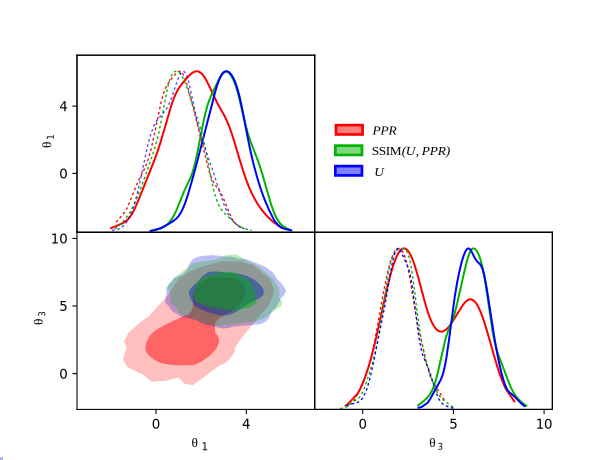
\includegraphics[width=.9\linewidth]{./illustrations/convergence.pdf}
\end{center}. In the same environment,
Gaussian under SSPR finishes faster and gets the right
answer. Under the same circumstances PPR inside SSPR also finishes
faster.

Choosing which one to include is like choosing your favourite
child. I could make the case that SSPR makes the simulation more
robust if wrapped inside PPR. On the other hand SSPR doesn't need
PPR. Maybe give Hobson and Feroz some credit here. I'm already
being overly negative about their discovery, even though my
discovery is based on theirs. PPR it is then. 

\subsubsection{{\bfseries\sffamily DONE} Project presentations.}
\label{sec:org20c439b}
According to Charles Smith we need to present our findings. 

update: Meeting is scheduled. 

\subsubsection{{\bfseries\sffamily DONE} e-mail Dr Handley about findings.}
\label{sec:org0d96bbd}

\subsection{Week 3}
\label{sec:orgc89ba1a}

\subsubsection{{\bfseries\sffamily DONE} Add Kullback-Leibler Divergence}
\label{sec:org656621a}
Kullbakc leibler divergence is useful but only marginally
so. Kullback Leibler from prior to posterior indicates performance
up to a point. 

PolyChord may converge faster for a stronger bias: e.g. if the
prior is sharply peaked at the origin. In that case
\(\mathcal{D}\) is larger but run-time is smaller.





\subsubsection{{\bfseries\sffamily DONE} Install Cosmochord.}
\label{sec:orga3b9b13}
Need \href{https://cosmologist.info/cosmomc/readme\_planck.html}{external Planck likelihood}. 

\subsubsection{{\bfseries\sffamily DONE} Install on Cluster}
\label{sec:org31e00bf}
Planck is typical academic abandonware. They have a ``python''
script that installs the dependencies called \texttt{waf}. In their
wizdom, they decided that they can do a better job than either
pypi, or conda. They wrote their own package manager that
downloads an outdated dependency if it can't find it (which it
can't because if you think and it can't. Because if you think
that writing your own package manager is a good idea, you're
really too stupid to do it properly.  find it, because people who
do pip and conda, don't abandon their software and move on.

As this may be read by someone who's writing academic code; the
proper procedure is telling the end-user that they need packages
x, y and z. If you're writing a package and it needs a package
manager, and you're not thinking of maintaining it -- Don't write
a package manager! Mainly because I don't think you'd bother to
check the venv, and update the download links. Also, you're
probably thinking that either pip or conda can't do what you need
them to do\ldots{} So you don't ask. 

This is at least six hours of wasted time, that could have been
avoided if people were not in the sweet-spot of writing difficult
to replicate, but at the same time completely unmaintained and
under-developed code. This is why I insist on \textbf{\textbf{proper}} software
engineering techniques! 

Also! Keep Science away from Python. It's design philosophy 'we're
all consenting adults', basically means that people do however,
whatever and there's no responsibility. Python is a unique
language: it has a few surface-level good ideas, a bunch of
terrible ones, and is moderated by people that clearly have no
idea what they're doing. That latter point is especially painful,
as for some reason they thought that creating a breaking change to
Python 3 was a good idea, yet they were unable to phase out
python2, and after all of that, they thought that keeping the
names of packages the same was not going to backfire.

The bigger problem is that people are seduced by the mild
syntactic sugar of python. Big projects are dragged down by the
cesspool of moronic design. It's giving me nightmares at this
point.

The project report guideline asks us to think of ways that could
make this easier. My suggestions. Don't use python. Don't! All the
time you save by avoiding the curly braces is being paid for in
sleep-deprived tortured people that just want to get their degree
done with. I'm fed up with Cobaya's overengineered nonsense. I
wanted to use CosmoChord to avoid Python at all costs. It doesn't
work. Because Python is used there as well. It's 2am. I'm trying
to figure out why pip swears that astropy is installed. While at
the same time no version of python seems to detect it. If that
wasn't enough; there's 17 version of pip on the cluster. I don't
know which one to use to install that damn thing! I shouldn't have
to know!

ANd the worst part is, people assume that writing python code is
easy, because of all the light-weight stuff. If I told someone
that I was stuck for an entire 24 hours trying to fix a build on a
cluster people would say "how hard can it be". Just pip install?
Right? 

Eventual workaround
\begin{verbatim}
module load python@3.8
sudo /usr/local/software/master/python/3.8/bin/python -m ensurepip 
module purge
module load python
/usr/local/bin/python -m ensurepip 
/usr/local/bin/python -m pip install astropy cython 
\end{verbatim}
Notice that I had to use a python3 pip to install a python2
pip. Naturally this is just stupidity.

\section{Notes}
\label{sec:orga7b8a26}
\subsection{Michaelmas Term}
\label{sec:org1542546}

Doing some research about the subject. 


\subsubsection{Terminology}
\label{sec:org71d0fda}

Prior - \(P(\theta | M)\)
Likelihood - \(P(M, \theta | Data)\)

Posterior - \(P(\theta | \text{Data})\)
Evidence - \(P(Model | Data)\)

Bayes' theorem says that 

\[Likelihood \times Prior = Posterior \times Evidence\]

So can use this to find the parameter values of a model, + the
likelihood that the model fits the data at all.


\subsubsection{How does nested sampling work}
\label{sec:org5de9bb3}

\begin{enumerate}
\item Skilling's paper
\label{sec:orged9b68d}

\cite{skilling2006}

Nested Sampling is a machine learning technique that allows to do Bayesian parameter estimation. 

Fitting a line to data is an example of a parameter fitting model. 

Set \(\chi^{2} \triangleq \sum_{i} \left(\frac{y_{i} - f(x_{i}, \theta)}{\sigma_{i}} \right)\). We need to ask a question, how likely is the data observed, given that the model is true, and the Model parameters have the given values. The probability is usually given by a Gaussian (or normal distribution). 

\[ 
	 L = \frac{1}{N} \exp{\left[ - \chi^{2}\right]}
	 \]

So what we need to do for Nested Sampling to work, is to
provide a model for estimating the fit to the hypothesis -
likelihood, and a prior.

The likelihood, or how likely is the value of data given the
model and the parameters, reflects how we expect the
fluctuations to develop. Many distributions are possible, but
due to the Central Limit theorem, best choice would be a
Normal (Gaussian) distribution.

The prior represents our prior knowledge of the original
parameters. For example, if we know nothing about the
possible model parameters, we can expect a uniform
distribution within constraints. These constraints may be
artificial (for example, we may only be interested in model
parameters that are within machine-representable floating
point numbers), or natural (the Hubble parameter is
positive).

If we know more about the model parameters, that information
can also be presented as a guideline for parameter
inference. For example if we have done parameter estimation
of the same model, using a different set of data; the
posterior of the aforementioned investigation can be used
directly as the prior for this run.

Nested sampling exploits that extra data to converge upon the
so-called typical set; which represents the data that has
statistically significant phase volume. The latter point can
be understood intuitively.

More accurate or tight constraints on the true data should
lead to better convergence time. Ideally the convergence to
the posterior of a distribution is the fastest, as this
minimises the number of errors, and given a suitable sampling
algorithm should lead to few wasted computations.


\begin{enumerate}
\item {\bfseries\sffamily TODO} Phase volume example.
\label{sec:orgea9149b}
\end{enumerate}





\item Notes on the Algorithm itself:
\label{sec:orgafc45ff}

Rasterising the phase space is too computationally
ineffective, as for a model with 27 parameters, the space
would be 27 dimensional. This leads to many quirks of
geometry and counter-intuitive outcomes, that will be touched
on later.

We must first select a number of live points randomly from
the phase space, usually taken to a be a hypercube with edge
length normalised to 1.

For each point one expects there to be a locus of points with
the exact same likelihood. This locus is often connected, and
so in analogy with isotherms it is often referred to as the
iso-likelihood contour.

Then one selects the least likely point and picks according
to some algorithm, a point of higher likelihood. The original
point is now referred to as dead, while the new point is
added to the set of live points.

This process is then repeated until we have reached a typical
set. This is often determined by estimating the \emph{evidence}
contained outside each contour (since the points are picked
at random, if we have n\(_{\text}\)\{live\} points, each contour will
statistically include \frac{1}\{n\(_{\text}\)\{live\}\} of the total
phase volume).


\item Piecewise power repartitioning notes.
\label{sec:org5e3e234}
Are these issues you're encountering for the mixture model, or the
temperature-dependent gaussian? (in the posterior repartitioning
paper, the pi\^{}\(\beta\) prior is terms 'power posterior repartitioning', so
we should refer to it as that).

For the power posterior repartitioning, remember we're doing it with a
diagonal prior covariance, so everything is separable and Z(beta)
should be derived as described in the posterior repartitioning paper,
namely:

\(\tilde{\pi} = G[\mu,\sigma](\theta)^\beta / Z(\beta)\)

\[Z(\beta) = \int_a^b G[\mu,\sigma](\theta)^\beta d\theta\].  where \(G\) denotes a gaussian,
and a and b are the limits of the uniform distribution. This is
expressible using erf:

\begin{equation}
  Z(\beta) = \frac{erf(\frac{(b-\mu)}{\sqrt{2}} \sigma) - erf(\frac{(a-\mu)}{\sqrt{2}} \sigma)}{2}
\end{equation}



I've spent a bit of time thinking this morning, and have realised that
the mixture model is not quite as trivial as I had imagined.

To be clear, working in 1d for now, our normalised modified prior is
of the form:

\[\tilde{\pi}(\theta) = \beta U[a,b](\theta) + (1-\beta)G[mu,sigma](\theta)\]

where there will be a,b,\(\mu\),\(\sigma\) for each dimension. To compute the prior
transformation which maps x\(\in\)[0,1] onto \(\theta\), nominally we should do this
via the inverse of the cdf:
\begin{equation}
      F(\theta) = \frac{\beta (\theta-a)}{(b-a)} +
      (1-\beta) \frac{1}{2}\frac{1+erf(\theta-\mu)}{\sqrt{2}\sigma}
\end{equation}

Unfortunately \(x = F(\theta)\) is not invertible. There is another way
around mapping \(x\in[0,1]\).

In general, if you have a mixture of normalised priors: \[ \pi(\theta) = \sum_i
 A_i f_i(\theta)\]

\[\sum_i A_i = 1 \] where each \(f_i\) has an inverse CDF of \(\theta = F^{-1}_i(x)\)

one can define a piecewise mapping from \(x\in[0,1]\) thus:

\(\theta = F^{-1}_{i}\left(\frac{x-\alpha_{i-1}}{A_i}\right) : \alpha_{i-1} < x < \alpha_i\)

\[\alpha_i = \sum_j^{i} A_j\]

Basically this uses x to first choose which component of the mixture
is active (via the piecewise bit), and then rescales the portion of x
within that mixture to [0,1].

This method seems a little hacky at first, but the more I think about
it the more reasonable it seems. I would be interested to hear your
opinion, and we can discuss on Wednesday morning. Until then,
practically you should focus on the diagonal PPR approach, as that is
much more straightforward, and captures the essence of the method.


\item Data and Parameter covariance matrices.
\label{sec:org532f035}

To avoid having to generate data with a given distribution,
we can simply and directly use the Parameter covariance
matrix, for our toy models.

This basically means that instead of using the model's
functional form, we directly assume that the distribution is
of Gaussian nature. This we simply plug into the log
likelihood, and the rest of the algorithm proceeds as if we
had data and the functional form, and the \(chi^2\)
computation was done for free.


\begin{enumerate}
\item Correlated vs Uncorrelated Gaussian log likelihoods
\label{sec:orgb8fdb4c}


If the parameter covariance matrix is completely diagonal,
then the parameters are each individually Gaussian
distributed, with a standard deviation being the diagonal
element.

An arbitrary coupling can lead to covariance on the
off-diagonal. These mixtures can be unmixed by using either
Singular Value or eigenvalue decomposition of the covariance
matrix. This can be simply regarded as a coordinate
transform, a passive one at that. Consequently, a Gaussian
distribution in Loglikelihood takes the following form.

Let \(\vec{\mu}\) be the vector of mean values of Gaussian
distributed parameters \(\vec{\theta}\) (we shall drop the
vector). The corresponding parameter covariance matrix is
\(G_{i,j}\).

Therefore the corresponding loglilkelihood is

\[ 
	  \ln {\cal L} = -N - (\theta - \mu)^{T} G^{-1} (\theta - \mu)
	  \],
where the normalisation constant is given by 
\[
	  N = \frac{\det \left| 2\pi G \right|}{2}
	  \].
\end{enumerate}
\end{enumerate}



\subsection{Lent Term}
\label{sec:org27e618e}

\subsubsection{Polychord \textit{<2020-01-10 Fri>}}
\label{sec:orge375ab0}

Polychord is a nested sampling program that uses directional
slicing, which is not (citation needed) a form of rejection
sampling.

To run polychord one needs to do three things:

\subsubsection{\texttt{settings}}
\label{sec:orgd99f279}

which needs the number of dimesnions with which we're working,
(very procedural, probably a consequence of fortran-centric
implementation).

The Settings have information about the verbosity of the
system.

\begin{verbatim}
settings.feedback = 0
\end{verbatim}
seems to be a good default. 

Polychord can resume the older run, if instructed (rather by
default), so in order to have clean bench-marking do

\begin{verbatim}
settings.read_resume=False
\end{verbatim}

To control running-time vs precision trade-off, use 

\begin{verbatim}
settings.nlive=175
\end{verbatim}

Changing it to a lower value makes the program run faster. 

Another way to control termination is the 

\begin{verbatim}
settings.precision_target=0.1
\end{verbatim}

But we should normally not tinker with it. 

\subsubsection{logLikelihood}
\label{sec:org1e7216f}

This is essentially a \(\chi^2\), which represents the
probability of our data, given the model and the parameter
values.

We need to define it for each model. Ideally what it needs to
return is the normalised probability, but not giving it the
proper normalisation doesn't seem to affect the run-time, only
the result.

\subsubsection{Prior}
\label{sec:orgc1c0804}

This is a weird function. What this is called, probably has
nothing to do with what it actually is: it's taking a point in
a unit hypercube and maps it onto the real \(\theta\) values.

This function is where we can get most of our performance
uplift.

Ideally assuming that the \emph{real} prior is the posterior the
algorithm should converge the fastest. This should however
affect the loglikelihood calls, because we're re-scaling the
space.

I \textbf{\textbf{think}} that this simply means that the absolute value of
the \textbf{\textbf{loglikelihood}} is \textbf{\textbf{not a meaningful}} number.

\begin{enumerate}
\item UPDATE: it is meaningful. Just not without the prior.  \textit{<2020-02-14 Fri>}
\label{sec:org13d7bd2}
AutoPR relies on
\end{enumerate}


\subsubsection{Approaches to modelling systems.  \textit{<2020-01-17 Fri>}}
\label{sec:orga849bf0}
One way to model all of our systems is by looking at the \(\chi^2\) and dealing with generated data. While this is close
to what the system might actually do, this is not itself a
good solution, it's slow and it requires extra computations in
generating the data with the properties that we need.

Instead we might simply treat the system as if it was already
diagonalised in the model parameter space. So if our model has

\begin{equation}
  \mu =
  \begin{pmatrix}
    \mu_{0}\\
    \mu_{1}\\
    \vdots\\
    \mu_{n}
  \end{pmatrix}
\end{equation}

and 

\begin{equation}
  G =
  \begin{pmatrix}
    \sigma_{1}^2 & \sigma_{12}^2 & \cdots & \sigma_{1n}^2\\
    \vdots & \ddots &  \vdots & \vdots \\
     \sigma_{n1}^2 & \sigma_{n2}^2 & \cdots & \sigma_{n}^2
  \end{pmatrix}
\end{equation}

which is itself a gaussian assumption, we get the following: as our loglikelihood

\begin{equation}
  \ln {\cal {L}}  = - N - (\theta - \mu)^{T}G^{-1}(\theta-\mu)
\end{equation}

where \(N\) can be found by integrating a multivariate Gaussian. See handout for Phase Transitions: 

\begin{equation}
  N = \ln \det |2\pi G |
\end{equation}

this can be evaluated in one fell swoop using 

\begin{verbatim}
numpy.linalg.slogdet(2*pi*G)
\end{verbatim}

This allows us to do calculations in a fraction of the time. 


\subsubsection{Comparison of runs. \textit{<2020-01-24 Fri>}}
\label{sec:org4fe5e5a}

Planck data can be downloaded from (see references), and using
the following constraints, we can compute the misfit between
data.


\begin{center}
\includegraphics[width=.9\linewidth]{../LCDM-NS/toy-models/1/Comparison of run with uniform prior and paper.pdf}
\end{center}


This shows profound agreement, usingThe following constraints
on the parameters.

\begin{verbatim}
    planck_ranges = numpy.array(
	    [[0.019, 0.025],
	     [0.095, 0.145],
	     [1.03, 1.05],
	     [0.01, 0.4],
	     [2.5, 3.7],
	     [0.885, 1.04],
	     [0.9, 1.1],
	     [0, 200],
	     [0, 1],
	     [0, 10],
	     [0, 400],
	     [0, 400],
	     [0, 400],
	     [0, 400],
	     [0, 10],
	     [0, 50],
	     [0, 50],
	     [0, 100],
	     [0, 400],
	     [0, 10],
	     [0, 10],
	     [0, 10],
	     [0, 10],
	     [0, 10],
	     [0, 10],
	     [0, 3],
	     [0, 3]])


    samples = anesthetic.NestedSamples(root='./data.1908.09139/lcdm/chains/planck')
    fig, ax = samples.plot_2d(['logA', 'ns'])
    # plt.show()


    # params = samples.columns[:27]
    params = samples.columns[:27]
    Sig = samples[params].cov().values
    mu = samples[params].mean().values
    nDims = len(mu)

    # Run of the original

    args = {
	    'root_name': 'planck',
	    'm': mu,
	    's': Sig,
	    'likelihood': lambda x: gaussian_likelihood(x, mu, Sig),
	    # 'renew_plots': True,
	    'renew_plots': False,
	    'nLive': 2,
	    'prior': lambda x: uniform_prior_with_ranges(x, planck_ranges),
	    'ax': ax
    }
    exec_polychord(**args)

... 
    newSamples = anesthetic.NestedSamples(root='./chains/planck')
    newSamples.plot_2d(ax)

    plt.show()
    fig = plt.figure()
\end{verbatim}

\subsubsection{Automated Power Posterior Repartitioning. \textit{<2020-01-24 Fri>}}
\label{sec:org1b7d285}

Looking at \url{https://arxiv.org/pdf/1908.04655.pdf} we can see
that one can get better convergence if we use something called
the Automated posterior repartitioning.

We start with a Gaussian prior. 

\begin{equation}
  \pi(\theta) = G(\mu, \sigma) (\theta)
\end{equation}

We then introduce an extra parameter into our system: 

\begin{equation}
  \tilde{\theta} = \begin{pmatrix}
	\theta_{1}\\
	\downarrow\\
	\theta_{n}\\
	\beta
  \end{pmatrix}
\end{equation}

We then use this parameter to rescale the prior that we
originally had:

\begin{equation}
  \tilde{\pi}(\tilde{\theta}}) = \frac{{G(\mu, \sigma)(\theta)}^\beta}{Z_\pi(\beta)}
\end{equation}

And normalise it to one Having done that we need to keep the
posterior the same, so we need to rescale (citation needed)
the loglikelihood to account for this change.

\begin{enumerate}
\item When, how and why do repartitioning. \textit{<2020-02-19 Wed>}
\label{sec:org39516c6}

After multiple experiments I arrived at the following.

Running PolyChord with a Gaussian is \textbf{\textbf{not the same}} as what
we want to accomplish.

When we consider two different priors, a Uniform from
\((a,b)^\otimes n\) and a Gaussian given by an \(n\times n\)
matrix \(\sigma\).

The histogram of the loglikelihood calls and their results
will be different, it will differ due to the \emph{effective
volume} which each of those will occupy.

Naturally a Gaussian, even if it has the same effective
volume cannot simultaneously give the same evidence and the
same Posterior.

So we can ask two kinds of questions:

a) What is the Posterior given the prior that has a different
volume.

In this case the loglikelihood calls will cluster around
different values. This is a legitimate question to ask, but
it requires more information.

If we take a system where we don't have the extra information
about the location of the posterior peaks and their shape,
and plug in a prior that does, we're biasing the system, and
effectively \emph{fudging} the answer. This can in some cases be
useful, but it's not quite what the project aims to do.

So instead of asking what would our answer be with a
different prior, we ask a different question. What would our
answer be if our system was biased to picke the values that
\emph{suspect} are the correct posterior values, without that
affecting the posterior distribution and injecting extra
information that we don't have/ can't quantify.

This is a philosophical issue. Intuitively, if we have the
extra information it \emph{must} be reflected in the prior. It
can't otherwise. In fact by biasing the system, even if we
repartition the combination \({\cal L } \pi\) we can still
end up with a biased and therefore useless result.

In fact, my experiments clearly show this; if the Prior
corresponding to \emph{a} Gaussian which is not the same as the
posterior (has a different value of the mean), it can result
in the algorithm terminating and generating a completely
false posterior.

See \url{./toy-models/1/1.0 Example of parameter covariance.py/}. 

By doing repartitioning we allow our guess to be wrong,
without that affecting the outcomes: posterior and evidence.




\item Correlated and Uncorrelated Gaussian:\textit{<2020-02-03 Mon>}
\label{sec:org2704c91}


Knowing that the parameter covariance matrix, is usually
positive defininte, one can argue that the question of
whether or not the parameters in the model are correlated, or
completely uncorrelated (i.e. each has a single standard
deviation value) is moot.

We can always perform a linear operation that diagonalises
the parameter covariance matrix, and what the algorithm needs
to do is only to work with the uncorrelated Gaussians.

That of course is true, but some repartitioning schemes are
more sensitive to this fact, and can only work after the
coordinate transformation has been performed, which itself
adds to the complexity.


Other algorithms are more capable of doing this properly. 



\item 
\label{sec:org17aa4e6}
\end{enumerate}

\subsection{Easter "vacation"}
\label{sec:org1d719b0}

Notes at this stage already in the form of write-up. If detailed
history is needed, just refer to the git history of the
project-report.org.


\subsubsection{Cobaya settings \textit{<2020-03-18 Wed>}}
\label{sec:orgf7e8f72}
Hi all, I've cc'd Aleksandr who\ldots{}.

\begin{verbatim}
sampler:
  polychord:
   num_repeats: 2d
   blocking:
    - [1, [omega_b, omega_cdm, theta_s_1e2, tau_reio, logA, ns]]
    - [20, [A_planck, A_cib_217, xi_sz_cib, A_sz, ps_A_100_100, 
       ps_A_143_143, ps_A_143_217, ps_A_217_217, ksz_norm, gal545_A_100, 
       gal545_A_143, gal545_A_143_217, gal545_A_217, calib_100T, calib_217T, 
       galf_TE_A_100_143, galf_TE_A_143_217, galf_TE_A_100_217, 
       galf_TE_A_100, galf_TE_A_143, galf_TE_A_217]]
\end{verbatim}

\bibliographystyle{unsrt}
\end{document}